\documentclass{beamer}
\usepackage[utf8]{inputenc}
\usepackage{graphicx}
\author[Sowmya Vajjala]{Instructor: Sowmya Vajjala}

\title[LING 410X]{LING 410X: Language as Data}
\subtitle{Semester: Spring '18}

\date{1 February 2018}

\institute{Iowa State University, USA}
%%%%%%%%%%%%%%%%%%%%%%%%%%%

\begin{document}

\begin{frame}\titlepage
\end{frame}

\begin{frame}
\frametitle{Class Outline}
\begin{itemize}
\item Some R functions
\item Analyzing word frequencies, distribution of word usage throughout the text. %Chapter 3--4: 30min
\item Splitting a text using regular expressions and then analyzing word usage across parts. %30min.
\item target: instead of counting frequent words for entire text, we now learn to do chapter by chapter (i.e.,  answering questions such as: where does "Nora" appear more frequently in the play? what chapter has most references to lead character in novel X etc.)
\end{itemize}
\end{frame}

\begin{frame}
\frametitle{News: new book published on corpus analysis with R}
\begin{itemize}
\item Title: Corpus Linguistics and Statistics with R: Introduction to Quantitative Methods in Linguistics
\item Author: Guillaume Desagulier
\item Published by Springer, accessible in University network for free.
\item \url{https://link.springer.com/content/pdf/10.1007\%2F978-3-319-64572-8.pdf}
\item table of contents and quick summary: \url{https://mailman.uib.no/public/corpora/attachments/20180131/aab68a32/attachment.txt}
\end{itemize}
\end{frame}

\begin{frame}[fragile]
\frametitle{old stuff: revision}
\begin{itemize}
\item which() function: we used it to get line numbers matching a string.
\scriptsize
\begin{verbatim}
u <- c(1,2,3,3,4,5,6,66,7,7,8)
which(u ==3) #gives: 3, 4
u ==3 #what does that give, without which?
\end{verbatim} \pause \small
\item gsub() function: used for substitution within a string.
\scriptsize
\begin{verbatim}
gsub("[[:punct:]]", " ", dollshouse_string)
-replaces all punctuation with a space, in dollshouse_string
\end{verbatim} \small \pause
\item length() function - gives you length (Number of items) in a vector/list
\item seq() function (e.g., seq(1,10) - gives a vector with items 1 ... 10
\item rep() function (e.g., rep(1,10) - gives a vector with items 1 ... 1
\end{itemize}
\end{frame}

\begin{frame}[fragile]
\frametitle{new: few more simple functions}
\begin{itemize}
\item sum() function takes a numeric vector and returns its sum.
\begin{verbatim}
v4 = c(1,2,3,4)
sum(v4)
10
\end{verbatim}
\item unlist() function: converts list to a vector. \scriptsize
\begin{verbatim}
t <- strsplit("this is a string", " ")
t
unlist(t)
\end{verbatim}
\end{itemize}
\end{frame}

\begin{frame}[fragile]
\frametitle{new: apply() functions in R}
\begin{itemize}
\item apply functions in R (lapply, sapply, vapply etc. ) are used for looping through of lists, vectors, and other such structures in R.
\item When are they used: typically used instead of writing loops.
\item one of these: lapply - you want to perform some operation on a list, and get back the output as another list. 
\pause \scriptsize \begin{verbatim}
v1 = c("This", "is", "an", "example")
v2 = c("This", "is", "another", "sentence")
v3 = c("Third", "string", "for", "this", "example")
temp = list(strsplit(v1, " "),strsplit(v2, " "),strsplit(v3, " "))
lapply(temp, '[', 2) #gives me all 2nd items within each item in temp.
\end{verbatim} \small
\item We can also write our own functions where we have that square bracket. More on that next week or later.
\end{itemize}
\end{frame}

\begin{frame}
\frametitle{}
\Large Analyzing word distribution throughout a text
\\ \small (based on Chapter 4 of the textbook)
\end{frame}

\begin{frame}[fragile]
\framesubtitle{Let us quick look at this code from Week 2}
\tiny
\begin{verbatim}
english <- scan("DollsHouse-Eng.txt", what = "character", sep = "\n")
english.start <- which (english ==  "DRAMATIS PERSONAE")
english.end <- which (english == "(The sound of a door shutting is heard from below.)")
dollshouse_text <- english[english.start:english.end]
dollshouse_string <- paste(dollshouse_text, collapse = " ")
dollshouse_string <- tolower(dollshouse_string)
dollshouse_string <- gsub("[[:punct:]]", " ", dollshouse_string)
dollshouse_string <- gsub(" +", " ", dollshouse_string)
dollshouse_words <-strsplit(dollshouse_string, "\\W")
sorted_wordfreqs_dollshouse <-sort(table(dollshouse_words), decreasing = TRUE)
\end{verbatim}
\normalsize At the end, what do you expect to see in sorted\_wordfreqs\_dollshouse? 
\\ (note: there are minor differences from what I used before - but nothing extremely new!)
\end{frame}

\begin{frame}[fragile]
\frametitle{What do you think the following lines will show as output?}
Let us go line by line: 
\footnotesize
\begin{verbatim}
length(sorted_wordfreqs_dollshouse)
sum(sorted_wordfreqs_dollshouse)
sorted_wordfreqs_dollshouse["doll"]
sorted_wordfreqs_dollshouse["he"]/sorted_wordfreqs_dollshouse["she"]
sorted_wordfreqs_dollshouse[1:10]
plot(sorted_wordfreqs_dollshouse[1:10], type="b")
\end{verbatim}
\end{frame}

\begin{frame}[fragile]
\frametitle{Raw counts to relative frequencies}
The table of words and their frequencies contains raw counts of the number of times a word appeared in this text. Let us say I want to convert this into counts showing: "number of times I will see a word for every 100 words"
\tiny
\begin{verbatim}
sorted_wordfreqs_dollshouse_100 <- 100 * (sorted_wordfreqs_dollshouse)/ sum(sorted_wordfreqs_dollshouse)
sorted_wordfreqs_dollshouse["the"]
sorted_wordfreqs_dollshouse_100["the"]
\end{verbatim}
\normalsize Remember "vector recycling" and vector division from your swirl lessons? We are using them here to do something useful. 
\\ What will happen if I plot with these new counts instead of raw counts?
\tiny \begin{verbatim}
plot(sorted_wordfreqs_dollshouse_100[1:10], type="b")
\end{verbatim}
\end{frame}

\begin{frame}
\frametitle{Disperson Plots}
\begin{itemize}
\item We saw how to know how frequently a word is used in a text.
\item We also saw how to compare two words in terms of their frequencies. \pause
\item Let us say I now want to create plots showing where a word occurs in the text - where is it more frequent, less frequent etc.
\item Dispersion plots are useful for doing this kind of analysis. \pause
\item X-axis: shows progression of the text. Let us say progression is shown from first word to last word of the entire text.
\item Y-axis: In this case, we are only noting presence/absence of a word throughout the text. So, that is our Y-axis
\end{itemize}
\end{frame}

\begin{frame}[fragile]
\frametitle{How to create a dispersion plot?}
\begin{enumerate}
\item Step 0: create a sequence vector for the number of words in the text (what is a sequence vector?) \pause
\item Step 1: get all locations of occurrence of a word (e.g., "is")
\item Step 2: Have a output vector that has the same dimension as sequence vector from Step 0. 
\item Step 3: Replace the locations where we see the word (is) in output with 1.
\end{enumerate}
\end{frame}

\begin{frame}[fragile]
\frametitle{}
\tiny
\begin{verbatim}
dollshouse_words_vector <- unlist(dollshouse_words)
progress <- seq(1:length(dollshouse_words_vector)))
nora <- which(dollshouse_words_vector == "nora") 
nora_progression <- rep(NA, length(progress))
nora_progression[nora] <- 1
plot(nora_progression, main="Dispersion plot for word 'nora' in 'A Doll\'s House' play", 
        xlab="position in text", ylab="nora", type="h", ylim=c(0,1), yaxt = 'n')
\end{verbatim}
\normalsize You can do this with any word you want in the text. 
\end{frame}

\begin{frame}[fragile]
\frametitle{Let us do a little bit more}
\framesubtitle{Chapter 4.2}
\begin{itemize}
\item Let us take a book with Chapters, do start looking at how many times a word appears in each chapter, and plot again.
\item I am going to use Moby Dick that the author also uses in his examples. \pause
\item What do you think the following lines are doing?
\tiny
\begin{verbatim}
moby <- scan("mobydick.txt", what = "character", sep = "\n")
moby.start <- which (moby ==  "CHAPTER 1. Loomings.")
moby.end <- which (moby == "orphan.")
moby.actual <- moby[moby.start:moby.end]
moby.chap.positions <- grep("^CHAPTER \\d", moby.actual)
moby.actual[moby.chap.positions]
\end{verbatim}
\end{itemize}
\pause \normalsize moby.chap.positions is a vector that will hold line numbers of the lines matching the regular expression. So, the last line will print you the actual lines matching those line numbers. 
\end{frame}

\begin{frame}[fragile]
\frametitle{}
This will give us info about where the chapters are starting and ending.  But, how do we know what is the end of last chapter? \pause 
\\ One simple solution is to just look at the length of the vector. The last line should indicate the end of the last chapter. 
\tiny \begin{verbatim}
moby.last.position <- length(moby.actual)
moby.chap.positions <- c(moby.chap.positions, moby.last.position)
moby.actual[moby.chap.positions]
\end{verbatim}
\end{frame}

\begin{frame}
\frametitle{For loop and If condition}
\begin{itemize}
\item To go through chapter by chapter and count word frequencies instead of counting throughout the text, we need to change our approach a little bit.
\item We should use a for loop to tell R that you want to do the same analysis for each chapter instead of full text at once. \pause
\item "If" condition is similar to regular English. It just says: if condition X is met, do this.
\end{itemize}
\end{frame}

\begin{frame}[fragile]
\frametitle{Looping through the chapters of Moby Dick}
Let us slowly go through line by line.
\tiny
\begin{verbatim}
chapters.raw <- list()
for (i in 1:(length(moby.chap.positions) -1))
{
  titleline <- moby.chap.positions[i]
  title <- moby.actual[titleline]
  start <- titleline+1
  end   <- moby.chap.positions[i+1]-1
  chapter.lines <- moby.actual[start:end]
  chapter.string <- tolower(paste(chapter.lines, collapse = " "))
  chapter.string <- gsub(" +", " ", gsub("[[:punct:]]", " ", chapter.string))
  chapter.words <- unlist(strsplit(chapter.string, "\\W"))
  chapter.freqs <- table(chapter.words)
  chapters.raw[[title]] <- chapter.freqs
}
\end{verbatim}
\normalsize At the end of this, chapters.raw should have the words and their frequencies for each and every individual chapter!!
\end{frame}

\begin{frame}
\frametitle{What did we do so far?}
\begin{itemize}
\item We started with the aim of looking at the distribution of words chapter by chapter in Moby Dick.
\item We first split the text into chapters by using a regular expression.
\item Then, we wrote a "loop" that goes through each chapter, does the same set of actions:  
\begin{itemize}
\item get chapter start and end positions
\item get chapter text from full book based on these line positions 
\item lowercase text, remove punctuations
\item split the text into words
\item count frequencies of words for each chapter
\end{itemize}
\end{itemize}
\end{frame}

\begin{frame}
\frametitle{}
\begin{itemize}
\item At the end, we had chapters.raw, a big variable which contained all we wanted.
\item So, how do we get what we want from this??
\item Remember the discussion about vectors and lists from tuesday?
\end{itemize}
\end{frame}

\begin{frame}
\frametitle{Accessing List items}
\begin{itemize}
\item chapters.raw is a \textbf{list} where we stored data in the form: $chapters.raw\lbrack \lbrack title \rbrack\rbrack <- chapter.freqs$
\item So, how do we access the first chapter and its word frequency list here? - chapters.raw \lbrack \lbrack1\rbrack\rbrack
\item chapters.raw \lbrack \lbrack 1\rbrack \rbrack \lbrack"whale"\rbrack - What will this then give me? \pause
\item chapters.raw \lbrack \lbrack 1\rbrack \rbrack \lbrack 1\rbrack - what will this give me? \pause
\item chapters.raw \lbrack \lbrack 1\rbrack \rbrack \lbrack \lbrack 1\rbrack \rbrack - what will this give me? \pause
\end{itemize}
\end{frame}

\begin{frame}
\frametitle{What next?}
\begin{itemize}
\item Okay, we have some way of getting chapter wise frequencies of words now. 
\item How do we get them all at once, instead of writing that line one by one for each chapter like this: 
\\ chapters.raw \lbrack \lbrack 1\rbrack \rbrack \lbrack"whale"\rbrack
\\ chapters.raw \lbrack \lbrack 2\rbrack \rbrack \lbrack"whale"\rbrack
\\ .... .... 
\end{itemize}
\end{frame}

\begin{frame}
\frametitle{lapply}
\begin{itemize}
\item We want all occurrences of some word ("whale" in my example) from all chapters using chapters.raw. \pause
\item using lapply for that: $whaledetails <- lapply(chapters.raw, "\lbrack", "whale")$
\item What this is saying is: 
\begin{itemize}
\item Go through the elements of chapters.raw one by one  \\ (e.g., chapters.raw \lbrack \lbrack 1\rbrack \rbrack, chapters.raw \lbrack \lbrack 2\rbrack \rbrack etc)
\pause \item "\lbrack" says: for each of these element, do bracketed subsetting: \\ (e.g., chapters.raw \lbrack \lbrack 1\rbrack \rbrack \lbrack 1\rbrack or chapters.raw \lbrack \lbrack 1\rbrack \rbrack \lbrack "whale"\rbrack )
\item "whale" is an additional argument that says: look for the word "whale" in each of these bracketed subset of each element of chapters.raw
\\ (i.e., look only for these: chapters.raw \lbrack \lbrack 1\rbrack \rbrack \lbrack "whale"\rbrack, chapters.raw \lbrack \lbrack 2\rbrack \rbrack \lbrack "whale"\rbrack etc.)
\end{itemize}
\end{itemize}
\end{frame}

\begin{frame}
\frametitle{}
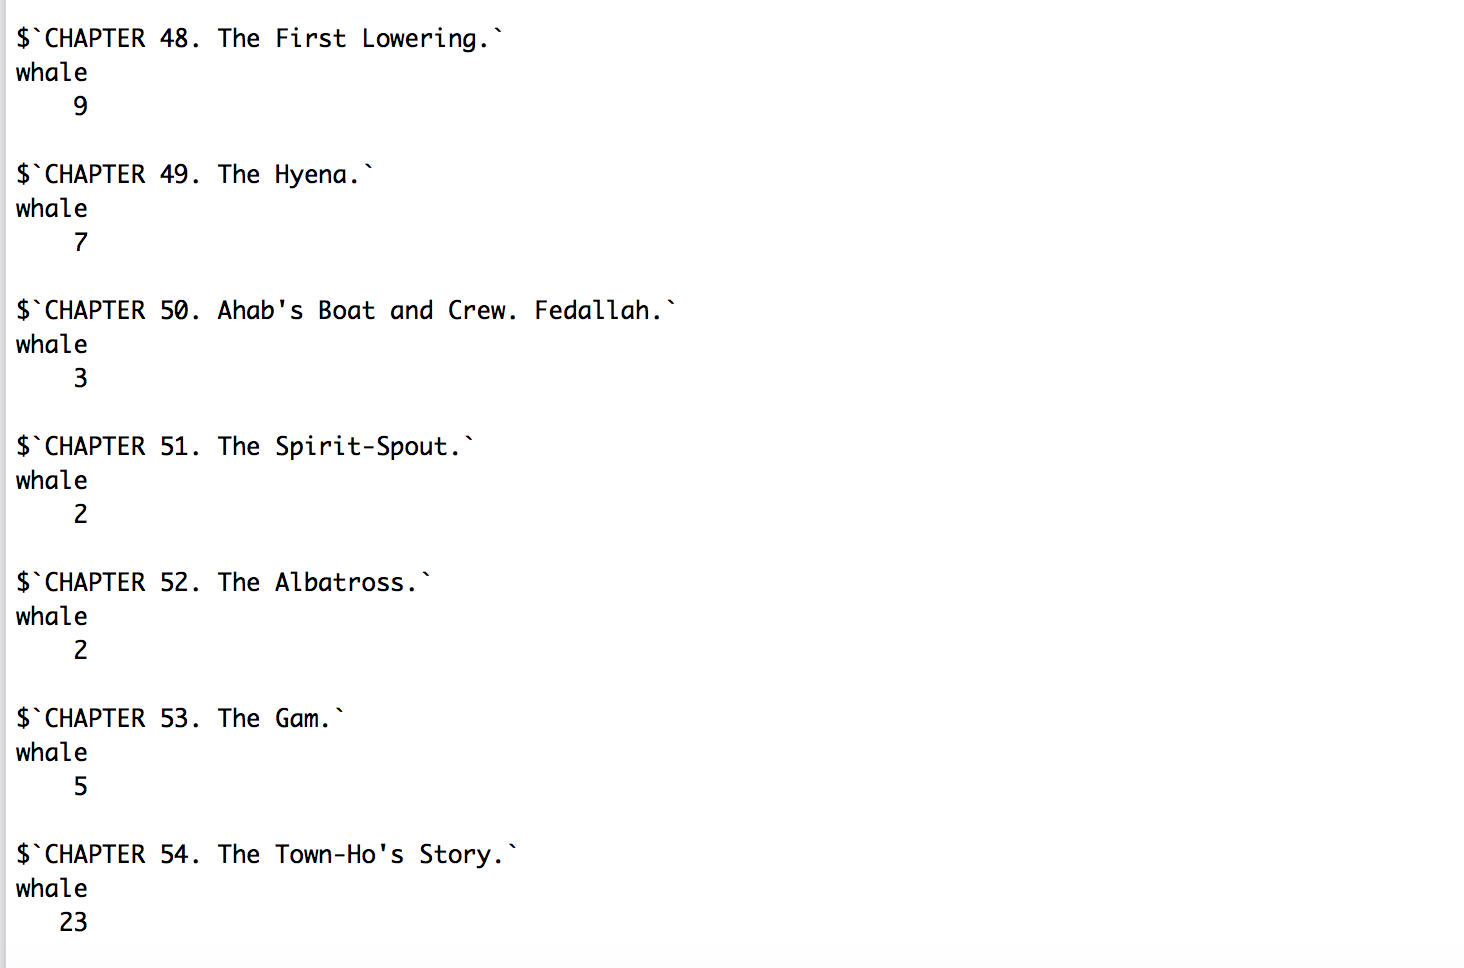
\includegraphics[width=0.8\textwidth]{whale.png}
\end{frame}

\begin{frame}[fragile]
\frametitle{what next?}
What is happening in this code snippet below?: 
\begin{verbatim}
whale_counts = c()
for (i in 1:length(whale))
{
  whale_counts[i] <- whale[[i]]
}
whale_counts
plot(whale_freqs_per_chap, type="h")
\end{verbatim}
\pause Note: There are several ways of doing this in R. The textbook describes another way of achieving this which requires you to know more about using functions like rbind(), do.call() etc. 
\end{frame}

\begin{frame}
\frametitle{Rest of the class}
Using R program, try to find out:
\begin{itemize}
\item How many chapters are there in David Copperfield (\url{http://www.gutenberg.org/files/766/766-0.txt})?
\item What chapter has the most number of occurrences of the name Murdstone?
\end{itemize}
\end{frame}

\begin{frame}
\frametitle{Next Week}
\begin{itemize}
\item Measures of lexical variety, and Hapax legomena (Chapters 6 and 7)
\item Searching for key words in context (Chapter 8)
\item ToDo: Read Chapter 6 and 7 by Tuesday. 
\item Note: I am leaving Chapter 5 out of my classwork.
\end{itemize}
\end{frame}

\end{document}

For classes next week:
Class 1: 
%\item Usage of R markdown to prepare reports of your analysis
%Chapter 5,6,7
%Ask if Darcy can do a quick presentation about Twitter? 


\begin{frame}
\frametitle{For the rest of this class}
\begin{itemize}
\item I uploaded a file called Twitter-2Feb2017.R in the Week4 folder in Blackboard. 
\item Open that file, and start running line by line. Follow the tutorial linked in the very first line 
\item I want you to work either individually or in groups, and practice the process of getting data from twitter - be it tweets or any other information.  \pause
\item If you already become familiar with all this, answer this question: If you search for the word "science" and get top 100 tweets, how many of them are Retweets?
\item You may want to look at how Retweets start. \pause
$length(grep("\hat{}RT\ ", tweets\_frame\$text))$
\end{itemize}
\end{frame}
